%%% Preamble
\documentclass[paper=a4, fontsize=11pt]{scrartcl}

%%AGREG0
\usepackage{float}
%\usepackage{geometry}
%\geometry{verbose,tmargin=2cm,bmargin=2cm,lmargin=2cm,rmargin=2cm,headheight=2cm,headsep=2cm}
%\geometry{verbose,tmargin=2cm,bmargin=2cm,lmargin=2cm,rmargin=2cm,headheight=2cm,headsep=2cm}

\usepackage[T1]{fontenc}
\usepackage{fourier}
\usepackage[utf8]{inputenc}
\usepackage[english]{babel}					% English language/hyphenation

\usepackage[protrusion=true,expansion=true]{microtype}	
\usepackage{amsmath,amsfonts,amsthm} % Math packages
\usepackage[pdftex]{graphicx}	
\usepackage{url}
\usepackage{import}

\usepackage[margin=2cm]{geometry}
\geometry{verbose,tmargin=2cm,bmargin=2cm,lmargin=2cm,rmargin=2cm,headheight=2cm,headsep=2cm}
% %%% Custom sectioning
\usepackage{sectsty}
\allsectionsfont{\normalfont \scshape}


%%% Custom headers/footers (fancyhdr package)
\usepackage{fancyhdr}
\pagestyle{fancyplain}
\fancyhead{}											% No page header
\fancyfoot[L]{}											% Empty 
\fancyfoot[C]{}											% Empty
\fancyfoot[R]{\thepage}									% Pagenumbering
\renewcommand{\headrulewidth}{0pt}			% Remove header underlines
\renewcommand{\footrulewidth}{0pt}				% Remove footer underlines
\setlength{\headheight}{13.6pt}


%%% Equation and float numbering
\numberwithin{equation}{section}		% Equationnumbering: section.eq#
\numberwithin{figure}{section}			% Figurenumbering: section.fig#
\numberwithin{table}{section}				% Tablenumbering: section.tab#


%%% Maketitle metadata
\newcommand{\horrule}[1]{\rule{\linewidth}{#1}} 	% Horizontal rule

%AGREGO PARA EJ 1
\usepackage{graphicx}
\usepackage{color} 
\usepackage[dvipsnames]{xcolor}
\colorlet{purple}{purple}

%/////////////////////////////////// AGREGO PARA EL EJ 2

    \usepackage{geometry} % Required to change the page size to A4
    \geometry{a4paper} % Set the page size to be A4 as opposed to the default US Letter

    \usepackage{mathtools, nccmath}
    
    \usepackage{tikz}
    \usetikzlibrary{matrix,calc}

    %isolated term
%#1 - Optional. Space between node and grouping line. Default=0
%#2 - node
%#3 - filling color
\newcommand{\implicantsol}[3][0]{
    \draw[rounded corners=3pt, fill=#3, opacity=0.3] ($(#2.north west)+(135:#1)$) rectangle ($(#2.south east)+(-45:#1)$);
    }


%internal group
%#1 - Optional. Space between node and grouping line. Default=0
%#2 - top left node
%#3 - bottom right node
%#4 - filling color
\newcommand{\implicant}[4][0]{
    \draw[rounded corners=3pt, fill=#4, opacity=0.3] ($(#2.north west)+(135:#1)$) rectangle ($(#3.south east)+(-45:#1)$);
    }

%group lateral borders
%#1 - Optional. Space between node and grouping line. Default=0
%#2 - top left node
%#3 - bottom right node
%#4 - filling color
\newcommand{\implicantcostats}[4][0]{
    \draw[rounded corners=3pt, fill=#4, opacity=0.3] ($(rf.east |- #2.north)+(90:#1)$)-| ($(#2.east)+(0:#1)$) |- ($(rf.east |- #3.south)+(-90:#1)$);
    \draw[rounded corners=3pt, fill=#4, opacity=0.3] ($(cf.west |- #2.north)+(90:#1)$) -| ($(#3.west)+(180:#1)$) |- ($(cf.west |- #3.south)+(-90:#1)$);
}

%group top-bottom borders
%#1 - Optional. Space between node and grouping line. Default=0
%#2 - top left node
%#3 - bottom right node
%#4 - filling color
\newcommand{\implicantdaltbaix}[4][0]{
    \draw[rounded corners=3pt, fill=#4, opacity=0.3] ($(cf.south -| #2.west)+(180:#1)$) |- ($(#2.south)+(-90:#1)$) -| ($(cf.south -| #3.east)+(0:#1)$);
    \draw[rounded corners=3pt, fill=#4, opacity=0.3] ($(rf.north -| #2.west)+(180:#1)$) |- ($(#3.north)+(90:#1)$) -| ($(rf.north -| #3.east)+(0:#1)$);
}

%group corners
%#1 - Optional. Space between node and grouping line. Default=0
%#2 - filling color
\newcommand{\implicantcantons}[2][0]{
    \draw[rounded corners=3pt, opacity=.3] ($(rf.east |- 0.south)+(-90:#1)$) -| ($(0.east |- cf.south)+(0:#1)$);
    \draw[rounded corners=3pt, opacity=.3] ($(rf.east |- 8.north)+(90:#1)$) -| ($(8.east |- rf.north)+(0:#1)$);
    \draw[rounded corners=3pt, opacity=.3] ($(cf.west |- 2.south)+(-90:#1)$) -| ($(2.west |- cf.south)+(180:#1)$);
    \draw[rounded corners=3pt, opacity=.3] ($(cf.west |- 10.north)+(90:#1)$) -| ($(10.west |- rf.north)+(180:#1)$);
    \fill[rounded corners=3pt, fill=#2, opacity=.3] ($(rf.east |- 0.south)+(-90:#1)$) -|  ($(0.east |- cf.south)+(0:#1)$) [sharp corners] ($(rf.east |- 0.south)+(-90:#1)$) |-  ($(0.east |- cf.south)+(0:#1)$) ;
    \fill[rounded corners=3pt, fill=#2, opacity=.3] ($(rf.east |- 8.north)+(90:#1)$) -| ($(8.east |- rf.north)+(0:#1)$) [sharp corners] ($(rf.east |- 8.north)+(90:#1)$) |- ($(8.east |- rf.north)+(0:#1)$) ;
    \fill[rounded corners=3pt, fill=#2, opacity=.3] ($(cf.west |- 2.south)+(-90:#1)$) -| ($(2.west |- cf.south)+(180:#1)$) [sharp corners]($(cf.west |- 2.south)+(-90:#1)$) |- ($(2.west |- cf.south)+(180:#1)$) ;
    \fill[rounded corners=3pt, fill=#2, opacity=.3] ($(cf.west |- 10.north)+(90:#1)$) -| ($(10.west |- rf.north)+(180:#1)$) [sharp corners] ($(cf.west |- 10.north)+(90:#1)$) |- ($(10.west |- rf.north)+(180:#1)$) ;
}

%Empty Karnaugh map 4x4
\newenvironment{Karnaugh}%
{
\begin{tikzpicture}[baseline=(current bounding box.north),scale=0.8]
\draw (0,0) grid (4,4);
\draw (0,4) -- node [pos=0.7,above right,anchor=south west] {y2 y1} node [pos=0.75,below left,anchor=north east] {w y3} ++(135:1);
%
\matrix (mapa) [matrix of nodes,
        column sep={0.8cm,between origins},
        row sep={0.8cm,between origins},
        every node/.style={minimum size=0.3mm},
        anchor=8.center,
        ampersand replacement=\&] at (0.5,0.5)
{
                       \& |(c00)| 00         \& |(c01)| 01         \& |(c11)| 11         \& |(c10)| 10         \& |(cf)| \phantom{00} \\
|(r00)| 00             \& |(0)|  \phantom{0} \& |(1)|  \phantom{0} \& |(3)|  \phantom{0} \& |(2)|  \phantom{0} \&                     \\
|(r01)| 01             \& |(4)|  \phantom{0} \& |(5)|  \phantom{0} \& |(7)|  \phantom{0} \& |(6)|  \phantom{0} \&                     \\
|(r11)| 11             \& |(12)| \phantom{0} \& |(13)| \phantom{0} \& |(15)| \phantom{0} \& |(14)| \phantom{0} \&                     \\
|(r10)| 10             \& |(8)|  \phantom{0} \& |(9)|  \phantom{0} \& |(11)| \phantom{0} \& |(10)| \phantom{0} \&                     \\
|(rf) | \phantom{00}   \&                    \&                    \&                    \&                    \&                     \\
};
}%
{
\end{tikzpicture}
}

%Empty Karnaugh map 2x4
\newenvironment{Karnaughvuit}%
{
\begin{tikzpicture}[baseline=(current bounding box.north),scale=0.8]
\draw (0,0) grid (4,2);
\draw (0,2) -- node [pos=0.7,above right,anchor=south west] {y2 y1} node [pos=0.7,below left,anchor=north east] {y3} ++(135:1);
%
\matrix (mapa) [matrix of nodes,
        column sep={0.8cm,between origins},
        row sep={0.8cm,between origins},
        every node/.style={minimum size=0.3mm},
        anchor=4.center,
        ampersand replacement=\&] at (0.5,0.5)
{
                      \& |(c00)| 00         \& |(c01)| 01         \& |(c11)| 11         \& |(c10)| 10         \& |(cf)| \phantom{00} \\
|(r00)| 0             \& |(0)|  \phantom{0} \& |(1)|  \phantom{0} \& |(3)|  \phantom{0} \& |(2)|  \phantom{0} \&                     \\
|(r01)| 1             \& |(4)|  \phantom{0} \& |(5)|  \phantom{0} \& |(7)|  \phantom{0} \& |(6)|  \phantom{0} \&                     \\
|(rf) | \phantom{00}  \&                    \&                    \&                    \&                    \&                     \\
};
}%
{
\end{tikzpicture}
}

%Empty Karnaugh map 2x2
\newenvironment{Karnaughquatre}%
{
\begin{tikzpicture}[baseline=(current bounding box.north),scale=0.8]
\draw (0,0) grid (2,2);
\draw (0,2) -- node [pos=0.7,above right,anchor=south west] {b} node [pos=0.7,below left,anchor=north east] {a} ++(135:1);
%
\matrix (mapa) [matrix of nodes,
        column sep={0.8cm,between origins},
        row sep={0.8cm,between origins},
        every node/.style={minimum size=0.3mm},
        anchor=2.center,
        ampersand replacement=\&] at (0.5,0.5)
{
          \& |(c00)| 0          \& |(c01)| 1  \\
|(r00)| 0 \& |(0)|  \phantom{0} \& |(1)|  \phantom{0} \\
|(r01)| 1 \& |(2)|  \phantom{0} \& |(3)|  \phantom{0} \\
};
}%
{
\end{tikzpicture}
}

%Defines 8 or 16 values (0,1,X)
\newcommand{\contingut}[1]{%
\foreach \x [count=\xi from 0]  in {#1}
     \path (\xi) node {\x};
}

%Places 1 in listed positions
\newcommand{\minterms}[1]{%
    \foreach \x in {#1}
        \path (\x) node {1};
}

%Places 0 in listed positions
\newcommand{\maxterms}[1]{%
    \foreach \x in {#1}
        \path (\x) node {0};
}

%Places X in listed positions
\newcommand{\indeterminats}[1]{%
    \foreach \x in {#1}
        \path (\x) node {X};
}

    \linespread{1.2} % Line spacing
    
    \setlength\parindent{0pt} % Uncomment to remove all indentation from paragraphs
    
   % \graphicspath{{/home/bzerol/VisualCode/ElectroIII/tp1-team-2/E2TP1}} % Specifies the directory where pictures are stored

%//////////////////////////////////// agrego para EJ 4
%\documentclass[english]{article}
%\usepackage[T1]{fontenc}
%\usepackage[latin9]{inputenc}
%\usepackage{geometry}
%\geometry{verbose,tmargin=2cm,bmargin=2cm,lmargin=2cm,rmargin=2cm,headheight=2cm,headsep=2cm}
%\usepackage{float}
%\usepackage{graphicx}

\makeatletter

%%%%%%%%%%%%%%%%%%%%%%%%%%%%%% LyX specific LaTeX commands.
%% Because html converters don't know tabularnewline
\providecommand{\tabularnewline}{\\}

%%%%%%%%%%%%%%%%%%%%%%%%%%%%%% User specified LaTeX commands.
\usepackage{babel}


\makeatother

\usepackage{babel}

%///////////////////////////// PARA EL EJ6
%\documentclass[english]{article}
%\usepackage[T1]{fontenc}
%\usepackage[latin9]{inputenc}
%\usepackage{geometry}
%\geometry{verbose,tmargin=3cm,bmargin=3cm,lmargin=3cm,rmargin=3cm,headheight=3cm,headsep=3cm}
%\usepackage{float}

%\makeatletter

%%%%%%%%%%%%%%%%%%%%%%%%%%%%%% LyX specific LaTeX commands.
%% Because html converters don't know tabularnewline
\providecommand{\tabularnewline}{\\}



\begin{document}

%\begin{titlepage}
    
\newcommand{\HRule}{\rule{\linewidth}{0.5mm}} % Defines a new command for the horizontal lines, change thickness here
    
\center % Center everything on the page
     
%----------------------------------------------------------------------------------------
%	HEADING SECTIONS
%----------------------------------------------------------------------------------------
    
\textsc{\LARGE Instituto Tecnológico de Buenos Aires}\\[2cm] % Name of your university/college
\textsc{\Large Electronica III}\\[1.5cm] % Major heading such as course name
\textsc{\large Trabajo Práctico N° 3}\\[0.5cm] % Minor heading such as course title
    
%----------------------------------------------------------------------------------------
%	TITLE SECTION
%----------------------------------------------------------------------------------------
    
\HRule \\[0.5cm]
{ \huge \bfseries Trabajo Práctico de Laboratorio Nr. 3}\\[0.4cm] % Title of your document
\HRule \\[2cm]
     
%----------------------------------------------------------------------------------------
%	AUTHOR SECTION
%----------------------------------------------------------------------------------------
    
\begin{minipage}{0.4\textwidth}
\begin{flushleft} \large
\emph{Grupo 2:}\\		%names
[.3cm]
Victor \textsc{Oh}\\
Leg. ???\\ 
[.3cm]
Ian \textsc{Diaz}\\
Leg. ???\\ 
[.3cm]
Benjamín Carlos \textsc{Lin}\\
Leg. 57242 \\ 
[.3cm]
Malena \textsc{Muller}\\
Leg. ???\\ 
[.3cm]
\end{flushleft}
\end{minipage}
~
\begin{minipage}{0.4\textwidth}
\begin{flushright} \large
%\emph{Profesor:} \\
%[.3cm]
%Pablo  \textsc{Cossutta}\\ % Supervisor's Name
%Alejandra \textsc{Weill} \\% Supervisor's Name
%Matías  \textsc{Salvati} % Supervisor's Name
\end{flushright}
\end{minipage}\\[2cm]
    
%----------------------------------------------------------------------------------------
%	DATE SECTION
%----------------------------------------------------------------------------------------
    
\vfill
{\large Entregado: 17 de Octubre de 2018}\\[2cm]
    
\vfill 
    
\end{titlepage}
%
%\pagenumbering{roman}
%\tableofcontents
%\newpage
%\pagenumbering{arabic}
%
%Test Text

\section{\color{olive}Exercise 1: }

\subsection{\color{purple}Mealy State Machine}

In the Mealy state machine, the output value not only depends on the state we are but also depends on the input values. This is to say the output could be represented as a function like $Z=f(X_1.....X_n,Q_1....Q_n)$ where Z: output, Q: State and X:Input event as could be visualize:

 \begin{figure}[h!]
        \centering
        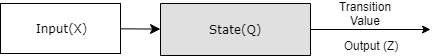
\includegraphics[scale=0.75]{Mealydiagram.png}
        \caption{\color{cyan}Mealy sate machine simple representation}
        \label{fig:ej1mealyr}
    \end{figure}

In this exercise, two sensors I and S function as input event to the state machine. Analyzing the possible states and event we obtain the following Mealy machine diagram:

 \begin{figure}[h!]
        \centering
        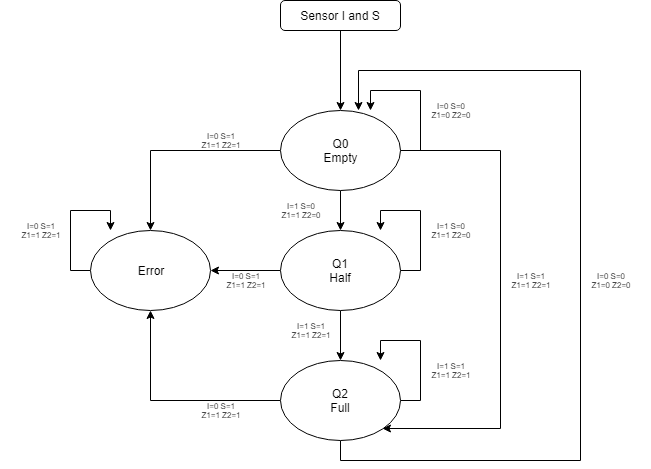
\includegraphics[scale=0.65]{ej1mealy.png}
        \caption{\color{cyan}Exercise 1: Mealy sate machine flow chart}
        \label{fig:ej1mealyd}
    \end{figure}

Which is represented as follow:

% Please add the following required packages to your document preamble:
% \usepackage{multirow}
\begin{table}[h!]
\centering
\begin{tabular}{|c|c|c|c|c|c|c|c|c|c|c|}
\hline
\multicolumn{3}{|c|}{\multirow{2}{*}{\textbf{State(Q)}}} & \multicolumn{8}{c|}{\textbf{Input(X)}} \\ \cline{4-11} 
\multicolumn{3}{|c|}{} & \multicolumn{2}{c|}{\textbf{I=0 S=0}} & \multicolumn{2}{c|}{\textbf{I=0 S=1}} & \multicolumn{2}{c|}{\textbf{I=1 S=0}} & \multicolumn{2}{c|}{\textbf{I=1 S=1}} \\ \hline
\textbf{Representation} & \textbf{Q2} & \textbf{Q1} & \textbf{Q2} & \textbf{Q1} & \textbf{Q2} & \textbf{Q1} & \textbf{Q2} & \textbf{Q1} & \textbf{Q2} & \textbf{Q1} \\ \hline
\textbf{Empty} & 0 & 0 & 0 & 0 & 0 & 1 & 1 & 0 & 1 & 1 \\ \hline
\textbf{Error} & 0 & 1 & 0 & 0 & 0 & 1 & 1 & 0 & 1 & 1 \\ \hline
\textbf{Half} & 1 & 0 & 0 & 0 & 0 & 1 & 1 & 0 & 1 & 1 \\ \hline
\textbf{Full} & 1 & 1 & 0 & 0 & 0 & 1 & 1 & 0 & 1 & 1 \\ \hline
\textbf{Output(Z)} & \textbf{Z1} & \textbf{Z2} & \textbf{0} & \textbf{0} & \textbf{1} & \textbf{1} & \textbf{1} & \textbf{0} & \textbf{1} & \textbf{1} \\ \hline
\end{tabular}
\caption{\color{cyan}Exercise 1: Mealy sate machine}
\end{table}

\pagebreak
So the logic circuit would be:

 \begin{figure}[h!]
        \centering
        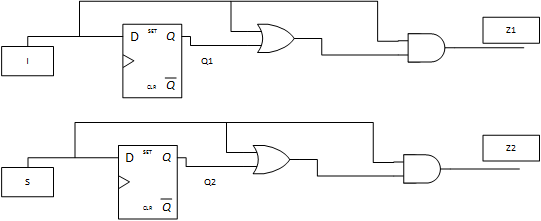
\includegraphics[scale=1]{ej1mealycircuit.png}
        \caption{\color{cyan}Exercise 1: Mealy logic circuit}
        \label{fig:ej1mealyld}
    \end{figure}

We can notice that the input event and the output event are the same which could make the $Z_N=X_N$ with N: the output or input number, but as mention be in the Mealy state machine the output $Z=f(X_1.....X_n,Q_1....Q_n)$, so we considered essential the use of sate in the circuit is dependent with the state and the input to have a clear view of being a Mealy state machine.

\subsubsection{\color{Orange}Simulation}

For the simulation of this stage machine, as the pump B1 and B2 alternate their function when $I = 1 y S = 0$ and for the activation of the pump that depends on output voltage is needed the following circuit is added:

 \begin{figure}[h!]
        \centering
        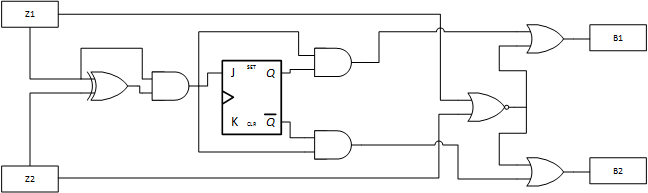
\includegraphics[scale=1]{ej1mealycircuitplus.png}
        \caption{\color{cyan}Exercise 1: Mealy additional logic circuit for the simulation}
        \label{fig:ej1mealylp}
    \end{figure}
    
Simulation the complete circuit in Verilog and testing the possibles values of input in Gtkwave the result was:

 \begin{figure}[h!]
        \centering
        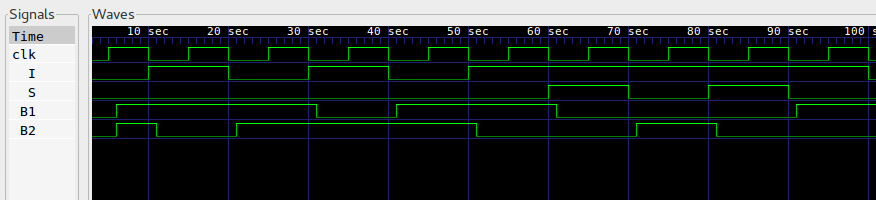
\includegraphics[scale=0.7]{ej1mealysim1.png}\\
        \vspace{0.2cm}
        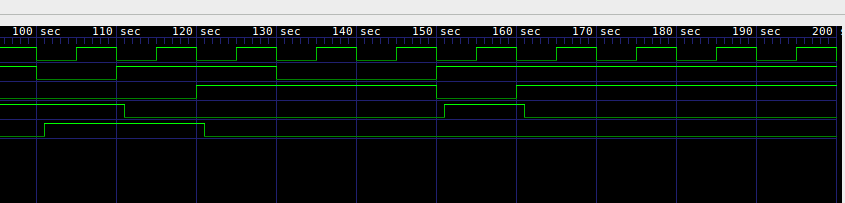
\includegraphics[scale=0.73]{ej1mealysim2.png}
        \caption{\color{cyan}Exercise 1: Simulation results}
        \label{fig:ej1mealyw}
    \end{figure}

%%%%%%%%%%%%%%%%%%%%%%%%%%%%%%%%%%%%%%%%
%Para Maleeeee
\pagebreak
Esto es Y1
\begin{center}
        \begin{Karnaugh}
            %cada 4 es una fila, la col 3 es la 4ta columna y 3fila es la 4 fila
            \contingut{
            0,0,1,0,
            0,X,X,X,
            1,0,0,0,
            0,X,X,X}
            \implicant{2}{6}{red}
            \implicant{8}{8}{green}
%            \implicant{12}{8}{orange}
%            \implicantdaltbaix[3pt]{1}{9}{blue}
            %\implicantcantons[2pt]{orange}
            %\implicantcostats{4}{14}{green}
        \end{Karnaugh}
    \end{center}

Y2
\begin{center}
        \begin{Karnaugh}
            %cada 4 es una fila, la col 3 es la 4ta columna y 3fila es la 4 fila
            \contingut{
            0,0,1,0,
            0,X,X,X,
            0,1,1,0,
            1,X,X,X}
            \implicant{2}{10}{red}
            \implicant{12}{14}{green}
%            \implicant{12}{8}{orange}
            \implicant{13}{9}{blue}
%            \implicantdaltbaix[3pt]{1}{9}{blue}
            %\implicantcantons[2pt]{orange}
            %\implicantcostats{4}{14}{green}
        \end{Karnaugh}
    \end{center}
  
  Y3  
\begin{center}
        \begin{Karnaugh}
            %cada 4 es una fila, la col 3 es la 4ta columna y 3fila es la 4 fila
            \contingut{
            0,0,0,0,
            0,X,X,X,
            0,0,0,1,
            0,X,X,X}
            \implicant{15}{11}{red}
%            \implicant{12}{14}{green}
%%            \implicant{12}{8}{orange}
%            \implicant{13}{9}{blue}
%            \implicantdaltbaix[3pt]{1}{9}{blue}
            %\implicantcantons[2pt]{orange}
            %\implicantcostats{4}{14}{green}
        \end{Karnaugh}
    \end{center}
    
    Z
    \begin{center}
        \begin{Karnaughvuit}
            %cada 4 es una fila, la col 3 es la 4ta columna y 3fila es la 4 fila
            \minterms{4}
        \maxterms{0,1,2,3}
        \indeterminats{5,6,7}
            \implicant{4}{6}{red}
%            \implicant{12}{14}{green}
%%            \implicant{12}{8}{orange}
%            \implicant{13}{9}{blue}
%            \implicantdaltbaix[3pt]{1}{9}{blue}
            %\implicantcantons[2pt]{orange}
            %\implicantcostats{4}{14}{green}
        \end{Karnaughvuit}
    \end{center}

%%%%%%%%%%%%%%%%%%%%%%%%%%%%%%%%%%%%%%%


\end{document}















%
%Having three different technology integrated circuits, 74HC02, 74HCT02 and 74LS02, we compare the noise margin between them and analyze the possible results when loading them with each other us follow:
%
% \begin{figure}[h!]
%        \centering
%        \includegraphics[scale=0.65]{circuit2.png}
%        \caption{\color{cyan}Logical circuit}
%        \label{fig:ej2circuit}
%    \end{figure}
%
%-Input(V): Input voltage; 
%-$X$: First component name; 
%-$Y$: Second component name; 
%-$q$: First result voltage; \\
%-$Q$: Final result
%
%	\subsection{\color{purple}Theoretically}
%	
%	 From the data-sheet of the components we obtain the following data when the power supply is $4.5V$ in the 74HC02 and 74HCT02 and around $5V$ for 74LS02:
%	 
%	 \begin{figure}[h!]
%        \centering
%        \includegraphics[scale=0.5]{dataaa2.png}
%        \caption{\color{cyan}Theoretical Noise Margin in Input and Output}
%        \label{fig:ej2thnm}
%    \end{figure}
%    
%    Within the mentioned values of power supply, the fanout of the components were: 74HC02 and 74HCT02 are 20, with $I_l =\pm1{\mu}A$ and $I_o=-20{\mu}A$; and 74LS02 is 80, with $I_l =0.1mA$ and $I_o=8mA$. As we load the components together, to avoid hurting the circuit, the maximum fanout allow shall be the minimum of the components, this is to say 20 in this case when we load HC with LS or HCT with LS. 
%    
%    Connecting the circuit like the figure \ref{fig:ej2cir} being $X$ the second column and $Y$ the forth column, analyzing the possible results would be:
%
%	\begin{center}
%	\hspace{2cm}\begin{table}[h!]
%	\begin{tabular}{llllllllllllllllllll} 
%	\cline{1-7}
%	\multicolumn{1}{|c|}{\multirow{2}{*}{Input(V)}}                                & \multicolumn{2}{c|}{74HC02}                                                       & \multicolumn{1}{c|}{\multirow{2}{*}{q}}          & \multicolumn{2}{c|}{74LS02}                                          & \multicolumn{1}{c|}{\multirow{2}{*}{Q}}             \\ \cline{2-3} \cline{5-6}
%	\multicolumn{1}{|c|}{}                                                 & \multicolumn{1}{c|}{Logic Input}        & \multicolumn{1}{c|}{Logic Output}       & \multicolumn{1}{c|}{}                            & \multicolumn{1}{c|}{Logic Input} & \multicolumn{1}{c|}{Logic Output} & \multicolumn{1}{c|}{}                               \\ \cline{1-7}
%	\multicolumn{1}{|c|}{0\textless{}V\textless{}1.35}                     & \multicolumn{1}{c|}{0}                  & \multicolumn{1}{c|}{1}                  & \multicolumn{1}{c|}{4.4\textless{}V\textless{}5} & \multicolumn{1}{c|}{1}           & \multicolumn{1}{c|}{0}            & \multicolumn{1}{c|}{0\textless{}V\textless{}0.5}    \\ \cline{1-7}
%	\multicolumn{1}{|c|}{\multirow{3}{*}{1.35\textless{}V\textless{}3.15}} & \multicolumn{1}{c|}{\multirow{3}{*}{?}} & \multicolumn{1}{c|}{\multirow{3}{*}{?}} & \multicolumn{1}{c|}{0\textless{}V\textless{}0.8} & \multicolumn{1}{c|}{0}           & \multicolumn{1}{c|}{1}            & \multicolumn{1}{c|}{2.7\textless{}V\textless{}5}    \\ \cline{4-7}
%	\multicolumn{1}{|c|}{}                                                 & \multicolumn{1}{c|}{}                   & \multicolumn{1}{c|}{}                   & \multicolumn{1}{c|}{0.8\textless{}V\textless{}2} & \multicolumn{1}{c|}{?}           & \multicolumn{1}{c|}{?}            & \multicolumn{1}{c|}{0.5\textless{}V\textless{}2.7}  \\ \cline{4-7}
%	\multicolumn{1}{|c|}{}                                                 & \multicolumn{1}{c|}{}                   & \multicolumn{1}{c|}{}                   & \multicolumn{1}{c|}{2\textless{}V\textless{}4.4} & \multicolumn{1}{c|}{1}           & \multicolumn{1}{c|}{0}            & \multicolumn{1}{c|}{0\textless{}V\textless{}0.5}    \\ \cline{1-7}
%	\multicolumn{1}{|c|}{3.15\textless{}V\textless{}5}                     & \multicolumn{1}{c|}{1}                  & \multicolumn{1}{c|}{0}                  & \multicolumn{1}{c|}{0\textless{}V\textless{}0.1} & \multicolumn{1}{c|}{0}           & \multicolumn{1}{c|}{1}            & \multicolumn{1}{c|}{2.7\textless{}V\textless{}5}\\ \cline{1-7}
%	\end{tabular}
%	\caption{\color{cyan}74HC02 load to 74LS02}
%	\label{fig:ej2thhctols}
%	\end{table}
%	\end{center}
%	
%	\begin{center}
%	\hspace{1cm}\begin{table}[h!]
%	\begin{tabular}{llllllllllllllllllll}
%	\cline{1-7}
%	\multicolumn{1}{|c|}{\multirow{2}{*}{Input(V)}} & \multicolumn{2}{c|}{74LS02} & \multicolumn{1}{c|}{\multirow{2}{*}{q}} & \multicolumn{2}{c|}{74HC02} & \multicolumn{1}{c|}{\multirow{2}{*}{Q}}  \\ \cline{2-3} \cline{5-6}
%	\multicolumn{1}{|c|}{} & \multicolumn{1}{c|}{Logic Input} & \multicolumn{1}{c|}{Logic Output} & \multicolumn{1}{c|}{} & \multicolumn{1}{c|}{Logic Input} & \multicolumn{1}{c|}{Logic Output} & \multicolumn{1}{c|}{}  \\ \cline{1-7}
%	\multicolumn{1}{|c|}{\multirow{2}{*}{0\textless{}V\textless{}0.8}} & \multicolumn{1}{c|}{\multirow{2}{*}{0}} & \multicolumn{1}{c|}{\multirow{2}{*}{1}} & \multicolumn{1}{c|}{2.7\textless{}V\textless{}3.15} & \multicolumn{1}{c|}{?} & \multicolumn{1}{c|}{?} & \multicolumn{1}{c|}{0.1\textless{}V\textless{}4.4}  \\ \cline{4-7}
%	\multicolumn{1}{|c|}{} & \multicolumn{1}{c|}{} & \multicolumn{1}{c|}{} & \multicolumn{1}{c|}{3.15\textless{}V\textless{}5} & \multicolumn{1}{c|}{1} & \multicolumn{1}{c|}{0} & \multicolumn{1}{c|}{0\textless{}V\textless{}0.1}  \\ \cline{1-7}
%	\multicolumn{1}{|c|}{\multirow{2}{*}{0.8\textless{}V\textless{}2}} & \multicolumn{1}{c|}{\multirow{2}{*}{?}} & \multicolumn{1}{c|}{\multirow{2}{*}{?}} & \multicolumn{1}{c|}{0.5\textless{}V\textless{}1.35} & \multicolumn{1}{c|}{0} & \multicolumn{1}{c|}{1} & \multicolumn{1}{c|}{4.4\textless{}V\textless{}5}  \\ \cline{4-7}
%	\multicolumn{1}{|c|}{} & \multicolumn{1}{c|}{} & \multicolumn{1}{c|}{} & \multicolumn{1}{c|}{1.35\textless{}V\textless{}2.7} & \multicolumn{1}{c|}{?} & \multicolumn{1}{c|}{?} & \multicolumn{1}{c|}{0.1\textless{}V\textless{}4.4}  \\ \cline{1-7}
%	\multicolumn{1}{|c|}{2\textless{}V\textless{}5} & \multicolumn{1}{c|}{1} & \multicolumn{1}{c|}{0} & \multicolumn{1}{c|}{0\textless{}V\textless{}0.5} & \multicolumn{1}{c|}{0} & \multicolumn{1}{c|}{1} & \multicolumn{1}{c|}{4.4\textless{}V\textless{}5}\\ \cline{1-7}
%	\end{tabular}
%	\caption{\color{cyan}74LS02 load to 74HC02}
%	\label{fig:ej2thlstohc}
%	\end{table}
%	\end{center}
%	
%	\begin{center}
%	\hspace{1cm}\begin{table}[h!]
%	\begin{tabular}{llllllllllllllllllll}
%	\cline{1-7}
%	\multicolumn{1}{|c|}{\multirow{2}{*}{Input(V)}} & \multicolumn{2}{c|}{74LS02} & \multicolumn{1}{c|}{\multirow{2}{*}{q}} & \multicolumn{2}{c|}{74HCT02} & \multicolumn{1}{c|}{\multirow{2}{*}{Q}}  \\ \cline{2-3} \cline{5-6}
%	\multicolumn{1}{|c|}{} & \multicolumn{1}{c|}{Logic Input} & \multicolumn{1}{c|}{Logic Output} & \multicolumn{1}{c|}{} & \multicolumn{1}{c|}{Logic Input} & \multicolumn{1}{c|}{Logic Output} & \multicolumn{1}{c|}{}  \\ \cline{1-7}
%	\multicolumn{1}{|c|}{0\textless{}V\textless{}0.8} & \multicolumn{1}{c|}{0} & \multicolumn{1}{c|}{1} & \multicolumn{1}{c|}{2.7\textless{}V\textless{}5} & \multicolumn{1}{c|}{1} & \multicolumn{1}{c|}{0} & \multicolumn{1}{c|}{4.4\textless{}V\textless{}5}  \\ \cline{1-7}
%	\multicolumn{1}{|c|}{\multirow{3}{*}{0.8\textless{}V\textless{}2}} & \multicolumn{1}{c|}{\multirow{3}{*}{?}} & \multicolumn{1}{c|}{\multirow{3}{*}{?}} & \multicolumn{1}{c|}{0.5\textless{}V\textless{}0.8} & \multicolumn{1}{c|}{0} & \multicolumn{1}{c|}{1} & \multicolumn{1}{c|}{4.4\textless{}V\textless{}5}  \\ \cline{4-7}
%	\multicolumn{1}{|c|}{} & \multicolumn{1}{c|}{} & \multicolumn{1}{c|}{} & \multicolumn{1}{c|}{0.8\textless{}V\textless{}2} & \multicolumn{1}{c|}{?} & \multicolumn{1}{c|}{?} & \multicolumn{1}{c|}{0.1\textless{}V\textless{}4.4}  \\ \cline{4-7}
%	\multicolumn{1}{|c|}{} & \multicolumn{1}{c|}{} & \multicolumn{1}{c|}{} & \multicolumn{1}{c|}{2\textless{}V\textless{}2.7} & \multicolumn{1}{c|}{1} & \multicolumn{1}{c|}{0} & \multicolumn{1}{c|}{0\textless{}V\textless{}0.1}  \\ \cline{1-7}
%	\multicolumn{1}{|c|}{2\textless{}V\textless{}5} & \multicolumn{1}{c|}{1} & \multicolumn{1}{c|}{0} & \multicolumn{1}{c|}{0\textless{}V\textless{}0.5} & \multicolumn{1}{c|}{0} & \multicolumn{1}{c|}{1} & \multicolumn{1}{c|}{4.4\textless{}V\textless{}5}\\ \cline{1-7}
%	\end{tabular}
%	\caption{\color{cyan}74LS02 load to 74HCT02}
%	\label{fig:ej2thlstohct}
%	\end{table}
%	\end{center}
%	
%	\begin{center}
%	\hspace{1cm}\begin{table}[h!]
%	\begin{tabular}{llllllllllllllllllll}
%	\cline{1-7}
%	\multicolumn{1}{|c|}{\multirow{2}{*}{Input(V)}} & \multicolumn{2}{c|}{74HCT02} & \multicolumn{1}{c|}{\multirow{2}{*}{q}} & \multicolumn{2}{c|}{74LS02} & \multicolumn{1}{c|}{\multirow{2}{*}{Q}}  \\ \cline{2-3} \cline{5-6}
%	\multicolumn{1}{|c|}{} & \multicolumn{1}{c|}{Logic Input} & \multicolumn{1}{c|}{Logic Output} & \multicolumn{1}{c|}{} & \multicolumn{1}{c|}{Logic Input} & \multicolumn{1}{c|}{Logic Output} & \multicolumn{1}{c|}{}  \\ \cline{1-7}
%	\multicolumn{1}{|c|}{0\textless{}V\textless{}0.8} & \multicolumn{1}{c|}{0} & \multicolumn{1}{c|}{1} & \multicolumn{1}{c|}{4.4\textless{}V\textless{}5} & \multicolumn{1}{c|}{1} & \multicolumn{1}{c|}{0} & \multicolumn{1}{c|}{0\textless{}V\textless{}0.5}  \\ \cline{1-7}
%	\multicolumn{1}{|c|}{\multirow{3}{*}{0.8\textless{}V\textless{}2}} & \multicolumn{1}{c|}{\multirow{3}{*}{?}} & \multicolumn{1}{c|}{\multirow{3}{*}{?}} & \multicolumn{1}{c|}{0.1\textless{}V\textless{}0.8} & \multicolumn{1}{c|}{0} & \multicolumn{1}{c|}{1} & \multicolumn{1}{c|}{2.7\textless{}V\textless{}5}  \\ \cline{4-7}
%	\multicolumn{1}{|c|}{} & \multicolumn{1}{c|}{} & \multicolumn{1}{c|}{} & \multicolumn{1}{c|}{0.8\textless{}V\textless{}2} & \multicolumn{1}{c|}{?} & \multicolumn{1}{c|}{?} & \multicolumn{1}{c|}{0.5\textless{}V\textless{}2.7}  \\ \cline{4-7}
%	\multicolumn{1}{|c|}{} & \multicolumn{1}{c|}{} & \multicolumn{1}{c|}{} & \multicolumn{1}{c|}{2\textless{}V\textless{}4.4} & \multicolumn{1}{c|}{1} & \multicolumn{1}{c|}{0} & \multicolumn{1}{c|}{0\textless{}V\textless{}0.5}  \\ \cline{1-7}
%	\multicolumn{1}{|c|}{2\textless{}V\textless{}5} & \multicolumn{1}{c|}{1} & \multicolumn{1}{c|}{0} & \multicolumn{1}{c|}{0\textless{}V\textless{}0.1} & \multicolumn{1}{c|}{0} & \multicolumn{1}{c|}{1} & \multicolumn{1}{c|}{2.7\textless{}V\textless{}5}\\ \cline{1-7}
%	\end{tabular}
%	\caption{\color{cyan}74HCT02 load to 74LS02}
%	\label{fig:ej2thhcttols}
%	\end{table}
%	\end{center}
%	
%	\pagebreak
%	
%	Therefore we expect when loading the components there will be are some irregularities in the Q output value when the input value aren't the recommended in the data-sheet. 
%
%	\subsection{\color{purple}Experimentally}
%	
%	Building the circuit in the figure \ref{fig:ej2cir} with the power supply to the integrated circuits equal to 5V with a square signal, altering its maximum value. The measured result were:
%	
%	\begin{figure}[h!]
%        \centering
%        \includegraphics[scale=0.19]{HC-LS-5V.png}\hspace{1cm}
%%        \includegraphics[scale=0.19]{HC-LS-2V.png}\\
%        \includegraphics[scale=0.19]{HC-LS-3V.png}\\
%		\vspace{0.2cm}
%%		\hspace{0.9cm}
%	   \includegraphics[scale=0.19]{HC-LS-2V.png}\hspace{1cm} 
%        \includegraphics[scale=0.19]{HC-LS-2p3V.png}
%        \caption{\color{cyan}74HC02 load to 74LS02}
%        \label{fig:ej2exhctols}
%    \end{figure}
%    
%    \begin{figure}[h!]
%        \centering
%        \includegraphics[scale=0.19]{LS-HC-5V.png}\hspace{1cm}
%        \includegraphics[scale=0.19]{LS-HC-3V.png}\\
%		\vspace{0.2cm}
%%		\hspace{0cm}
%        \includegraphics[scale=0.19]{LS-HC-1p5V.png}\hspace{1cm}
%         \includegraphics[scale=0.19]{LS-HC-0p7V.png}\\
%        \vspace{0.2cm}
%%		\hspace{0.9cm}
%        \includegraphics[scale=0.19]{LS-HC-1V.png}
%        \caption{\color{cyan}74LS02 load to 74HC02}
%        \label{fig:ej2exlstohc}
%    \end{figure}
%    
%%    \pagebreak
%    \begin{figure}[h!]
%        \centering
%        \includegraphics[scale=0.19]{LS-HCT-5V.png}\hspace{1cm}
%        \includegraphics[scale=0.19]{LS-HCT-3V.png}\\
%		\vspace{0.2cm}
%%		\hspace{0cm}
%        \includegraphics[scale=0.19]{LS-HCT-1p5V.png}\hspace{1cm}
%        \includegraphics[scale=0.19]{LS-HCT-0p7V.png}\\
%        \vspace{0.2cm}
%%		\hspace{0.9cm}
%        \includegraphics[scale=0.19]{LS-HCT-1p1V.png}
%        \caption{\color{cyan}74LS02 load to 74HCT02}
%        \label{fig:ej2exlstohct}
%    \end{figure}
%
%    \begin{figure}[h!]
%        \centering
%        \includegraphics[scale=0.18]{HCT-LS-5V.png}\hspace{1cm}
%        \includegraphics[scale=0.18]{HCT-LS-3V.png}\\
%		\vspace{0.2cm}
%%		\hspace{0.9cm}
%	   \includegraphics[scale=0.18]{HCT-LS-1p8V.png}\hspace{1cm}
%	   \includegraphics[scale=0.18]{HCT-LS-1V.png}\\
%	   \vspace{0.2cm}
%%		\hspace{0cm}
%%        \hspace{1cm}
%        \includegraphics[scale=0.18]{HCT-LS-0p6V.png}\hspace{1cm}
%        \includegraphics[scale=0.18]{LS-HCT-1p1V.png}
%        \caption{\color{cyan}74HCT02 load to 74LS02}
%        \label{fig:ej2exhcttols}
%    \end{figure}
%    
%    \pagebreak
%
%	Analyzing the results in $Q$ it is clear that the irregularities are odd to find, this could be because the manufacturer always leaves a bigger margin to ovoid conflicts within each unique component. Moreover as mention in the theoretical table when the input voltage isn't a logical input, in other words the supply voltage is in the prohibited zone because the circuit cannot decide if the the value of the voltage is low or high, the output value $q$ could mean something in the second component leading to misunderstandings or errors in the logical function. In the other hand, we can notice that using the HCT with the LS integrated circuits, their irregularity is lower in amplitude and not so define as HC with LS, cause their input noise margin are similar. 
%
%\end{document}